\documentclass[a4paper,12pt]{article}

\usepackage[utf8]{inputenc}
\usepackage[T1]{fontenc}
\usepackage[french]{babel}
\usepackage{graphicx}
\usepackage{hyperref}
\usepackage{geometry}
\usepackage{float}
\usepackage{xcolor}
\usepackage{tcolorbox}
\usepackage{fancyhdr}
\usepackage{titlesec}
\usepackage{enumitem}
\usepackage{fontawesome5}
\usepackage{tikz}
\usetikzlibrary{shapes,arrows,positioning}
\usepackage{caption}

% --- Configuration des Couleurs (Charte IUT/App) ---
\definecolor{primaryBlue}{RGB}{25, 113, 194} % Bleu Mantine
\definecolor{accentYellow}{RGB}{240, 140, 0} % Jaune Mantine
\definecolor{lightGray}{RGB}{248, 249, 250}

% --- Configuration des Marges ---
\geometry{hmargin=2cm,vmargin=2.5cm}

% --- En-têtes et Pieds de page ---
\pagestyle{fancy}
\fancyhf{}
\fancyhead[L]{\small \textcolor{primaryBlue}{\textbf{Skill Hub}}}
\fancyhead[R]{\small \textit{Guide Utilisateur}}
\fancyfoot[C]{\thepage}
\renewcommand{\headrulewidth}{0.4pt}
\renewcommand{\headrule}{\hbox to\headwidth{\color{primaryBlue}\leaders\hrule height \headrulewidth\hfill}}

% --- Styles des Titres ---
\titleformat{\section}
  {\color{primaryBlue}\normalfont\Large\bfseries\uppercase}
  {\thesection}{1em}{}[{\titlerule[0.8pt]}]
  
\titleformat{\subsection}
  {\color{accentYellow}\normalfont\large\bfseries}
  {\thesubsection}{1em}{}

% --- Boîtes d'Information ---
\newtcolorbox{infoBox}[1]{
  colback=lightGray,
  colframe=primaryBlue,
  title=#1,
  fonttitle=\bfseries,
  arc=4mm
}

% --- Configuration Images ---
\graphicspath{ {./capture/} }

% --- Méta-données ---
\title{Guide de Prise en Main : Skill Hub}
\author{Département TC - IUT Le Havre}
\date{\today}

\begin{document}

% --- PAGE DE GARDE ---
\begin{titlepage}
    \centering
    \vspace*{1cm}
    \begin{minipage}{0.45\textwidth}
        \centering
        
\includegraphics[height=2cm]{logo_iut}
    \end{minipage}
    \hfill
    \begin{minipage}{0.45\textwidth}
        \centering
        
\includegraphics[height=2cm]{logo_univ}
    \end{minipage}
    
    \vspace{2cm}
    
\includegraphics[width=0.4\textwidth]{1} % Logo ou capture d'accueil en guise de logo
    \vspace{2cm}
    
    {\color{primaryBlue} \Huge \textbf{SKILL HUB}} \\
    \vspace{0.5cm}
    {\Large \textit{Le pilotage intelligent de la formation}}
    
    \vspace{3cm}
    
    \begin{tcolorbox}[colback=accentYellow!10,colframe=accentYellow,width=0.8\textwidth,arc=2mm,boxrule=1pt]
        \centering
        \large \textbf{Guide de l'Enseignant}
    \end{tcolorbox}
    
    \vfill
    
    \textbf{IUT Le Havre - Département TC}\\
    Contact : \href{mailto:steeve.pytel@univ-lehavre.fr}{steeve.pytel@univ-lehavre.fr}\\
    \today
\end{titlepage}

\tableofcontents
\newpage

\section{Introduction}
Ce document est votre guide de référence pour la prise en main de \textbf{Skill Hub}, la nouvelle plateforme de gestion pédagogique du département TC.

Face aux défis de l'\textbf{Approche Par Compétences (APC)}, Skill Hub a été conçu pour transformer la gestion administrative en un véritable \textbf{pilotage pédagogique}. Cet outil centralise l'ensemble des informations relatives aux enseignements, aux étudiants et à l'évaluation des compétences, tout en favorisant la réflexivité des étudiants.

\begin{infoBox}{Accès Rapide}
    L'application est accessible depuis n'importe quel appareil (PC, Tablette, Smartphone) à l'adresse : \\
    \centerline{\Large \url{https://home.educ-ai.fr/app/}}
\end{infoBox}

\begin{figure}[H]
    \centering
    \fbox{
\includegraphics[width=0.9\textwidth]{1}}
    \caption{Interface d'accueil du Skill Hub}
\end{figure}

\section{Comprendre l'écosystème}

\subsection{Les rôles dans Skill Hub}
Pour garantir un suivi fluide, quatre profils d'utilisateurs interagissent sur la plateforme :

\begin{itemize}[label=\textcolor{primaryBlue}{\faUser}]
    \item \textbf{Directeur d'Études / Admin :} Pilote la structure globale, gère les affectations des intervenants et supervise la conformité du référentiel.
    \item \textbf{Enseignant / Tuteur :} Valide les acquis (AC/CE), suit l'avancement des étudiants dans sa ressource ou son groupe de tutorat.
    \item \textbf{Étudiant :} Acteur central de son parcours. Il dépose ses preuves de compétences (Médiathèque) et réalise son auto-évaluation.
    \item \textbf{Tuteur Entreprise :} Intervient via un \textbf{"Magic Link"} (sans compte à créer) pour évaluer le savoir-être de l'étudiant en fin de stage.
\end{itemize}

\subsection{Glossaire des concepts clés}
L'APC introduit une terminologie spécifique que Skill Hub intègre nativement :
\begin{description}
    \item[AC (Apprentissage Critique) :] Ce que l'étudiant doit savoir faire dans un contexte donné.
    \item[CE (Composante Essentielle) :] Les briques élémentaires qui constituent une compétence.
    \item[Ressource (R) :] Les cours théoriques et TD (le "savoir").
    \item[SAÉ :] Situations d'Apprentissage et d'Évaluation (projets professionnalisants).
\end{description}

\subsection{L'Architecture : Un triptyque intégré}
Skill Hub n'est pas un outil isolé. Il s'appuie sur trois piliers technologiques pour garantir une expérience sans couture :

\begin{center}
\begin{tikzpicture}[node distance=2cm, auto, thick, scale=0.8, every node/.style={scale=0.8}]
    \tikzstyle{block} = [rectangle, draw, fill=primaryBlue!10, text width=3.5cm, text centered, rounded corners, minimum height=1.5cm, draw=primaryBlue]
    \tikzstyle{line} = [draw, ->, thick, primaryBlue]
    
    \node [block, fill=primaryBlue!20] (hub) {\textbf{LE HUB}\\(Pilotage \& APC)};
    \node [block, fill=green!10, below left=of hub, draw=green!50!black] (nextcloud) {\textbf{NEXTCLOUD}\\(Gestion des fichiers)};
    \node [block, fill=purple!10, below right=of hub, draw=purple!50!black] (mattermost) {\textbf{MATTERMOST}\\(Communication)};
    
    \path [line] (hub) -- (nextcloud);
    \path [line] (hub) -- (mattermost);
\end{tikzpicture}
\end{center}

\begin{itemize}
    \item \textbf{Le Hub :} Le cerveau qui gère le référentiel, les notes et les parcours.
    \item \textbf{Nextcloud :} La "mémoire" où sont stockés les livrables et le portfolio.
    \item \textbf{Mattermost :} L'outil de discussion instantanée (Chat) pour les équipes.
\end{itemize}

\newpage
\section{Accès et Connexion}

L'authentification est conçue pour être transparente et sécurisée.

\subsection*{Procédure de connexion}
\begin{enumerate}
    \item Rendez-vous sur l'URL de l'application.
    \item Saisissez vos \textbf{identifiants académiques} (ENT).
    \item Cliquez sur "Se connecter".
\end{enumerate}

\begin{tcolorbox}[colback=red!5,colframe=red!75!black,title=Attention]
Si vous rencontrez un problème de connexion, vérifiez d'abord que votre accès à l'ENT de l'université fonctionne. Le Skill Hub utilise le même annuaire.
\end{tcolorbox}

\newpage
\section{Le Bloc Pilotage}
Le menu latéral gauche est votre outil de navigation principal. Le premier bloc, \textbf{Pilotage}, vous donne une vue d'ensemble de votre activité.

\subsection{Tableau de bord}
Dès la connexion, vous arrivez sur votre \textbf{Tableau de bord}. C'est votre espace personnel.

\textbf{Ce que vous y trouvez :}
\begin{itemize}[label=\textcolor{primaryBlue}{\textbullet}]
    \item Vos \textbf{Ressources} (cours, TD, TP) de l'année.
    \item Les \textbf{SAÉ} que vous encadrez ou supervisez.
    \item Les indicateurs de \textbf{suivi de stage}.
\end{itemize}

\begin{figure}[H]
    \centering
    \fbox{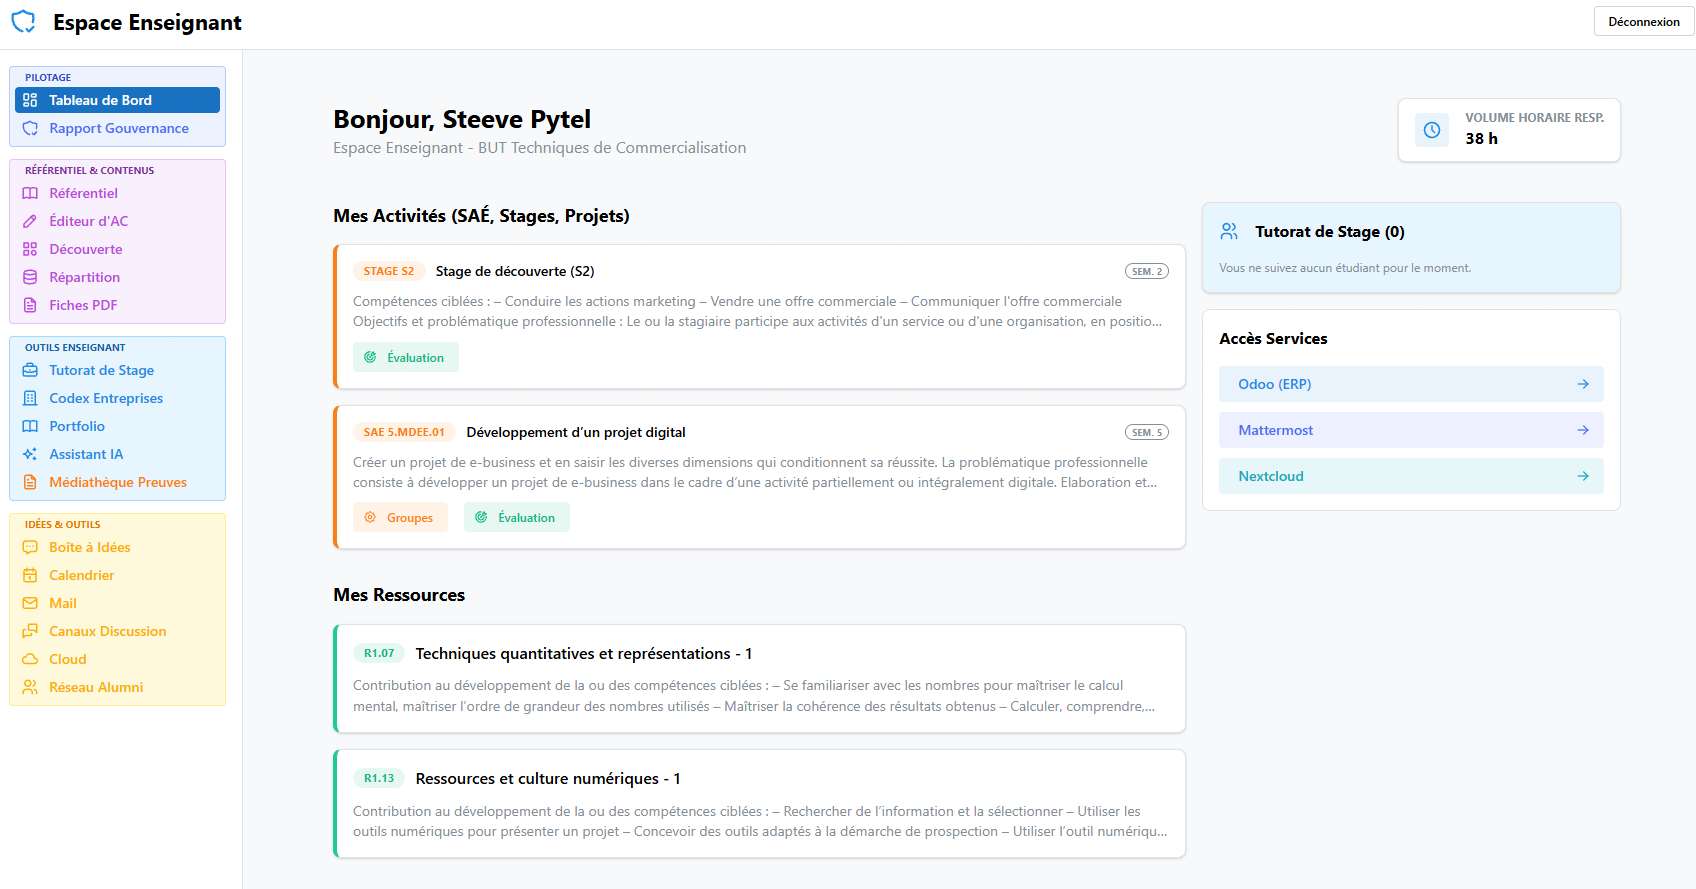
\includegraphics[width=0.85\textwidth]{2}}
    \caption{Tableau de bord : Vos modules en un coup d'œil}
\end{figure}

\subsection{Rapport de gouvernance}
Le rapport de gouvernance est l'annuaire fonctionnel du département. Il permet de savoir \textbf{``Qui fait quoi''**}.

\textbf{Usage clé :} Utilisez cet outil pour identifier rapidement les responsables de modules ou de SAÉ afin de coordonner vos interventions pédagogiques.

\begin{figure}[H]
    \centering
    \fbox{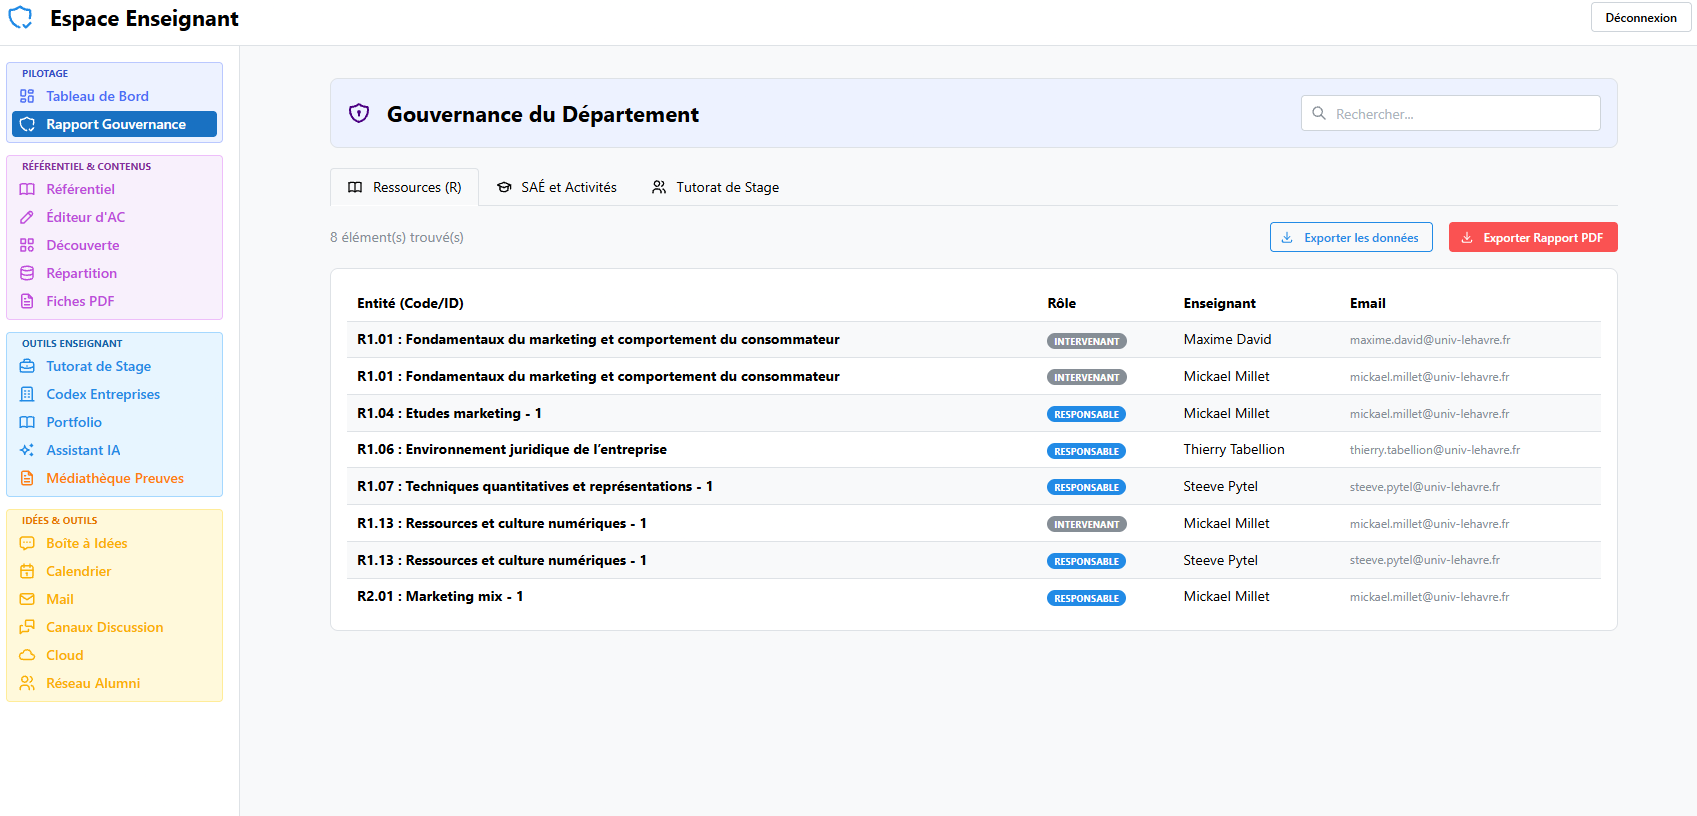
\includegraphics[width=0.85\textwidth]{3}}
    \caption{Vue globale des responsabilités pédagogiques}
\end{figure}

\newpage
\section{Le Bloc Référentiel \& Contenus}
Ce bloc est le cœur académique de l'application. Il contient la structure officielle du BUT TC.

\subsection{Référentiel \& Affectations}
Cette vue permet non seulement de consulter le programme, mais surtout de \textbf{gérer les équipes}.
En tant que responsable, c'est ici que vous affectez les intervenants aux différentes ressources.

\begin{figure}[H]
    \centering
    \fbox{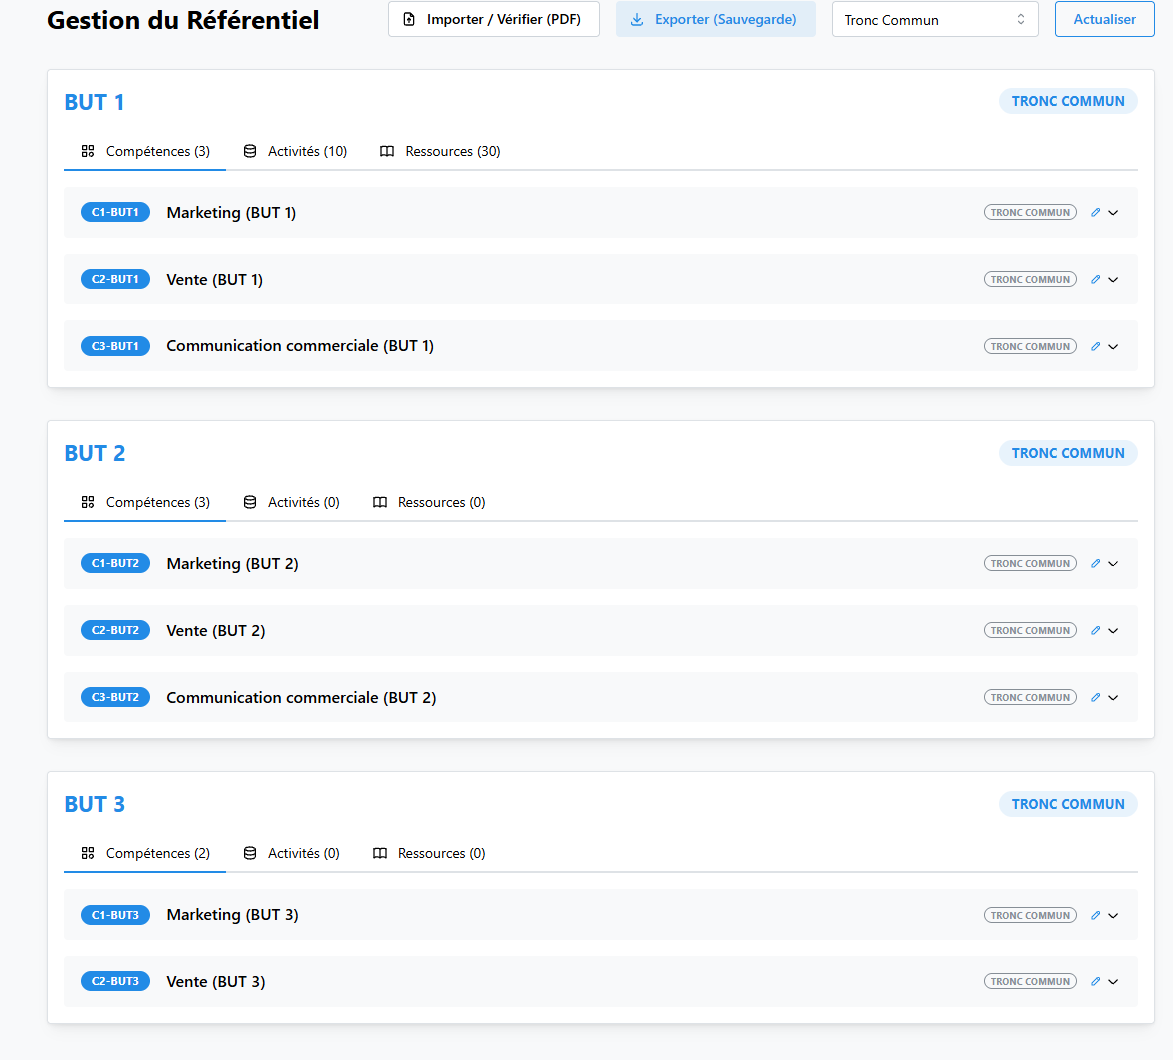
\includegraphics[width=0.85\textwidth]{4}}
    \caption{Gestion du référentiel et des équipes}
\end{figure}

\subsection{Éditeur d'AC (Apprentissages Critiques)}
L'outil de personnalisation par excellence. Il permet d'adapter les définitions nationales des AC aux réalités locales de nos projets et SAÉ.

\begin{figure}[H]
    \centering
    \fbox{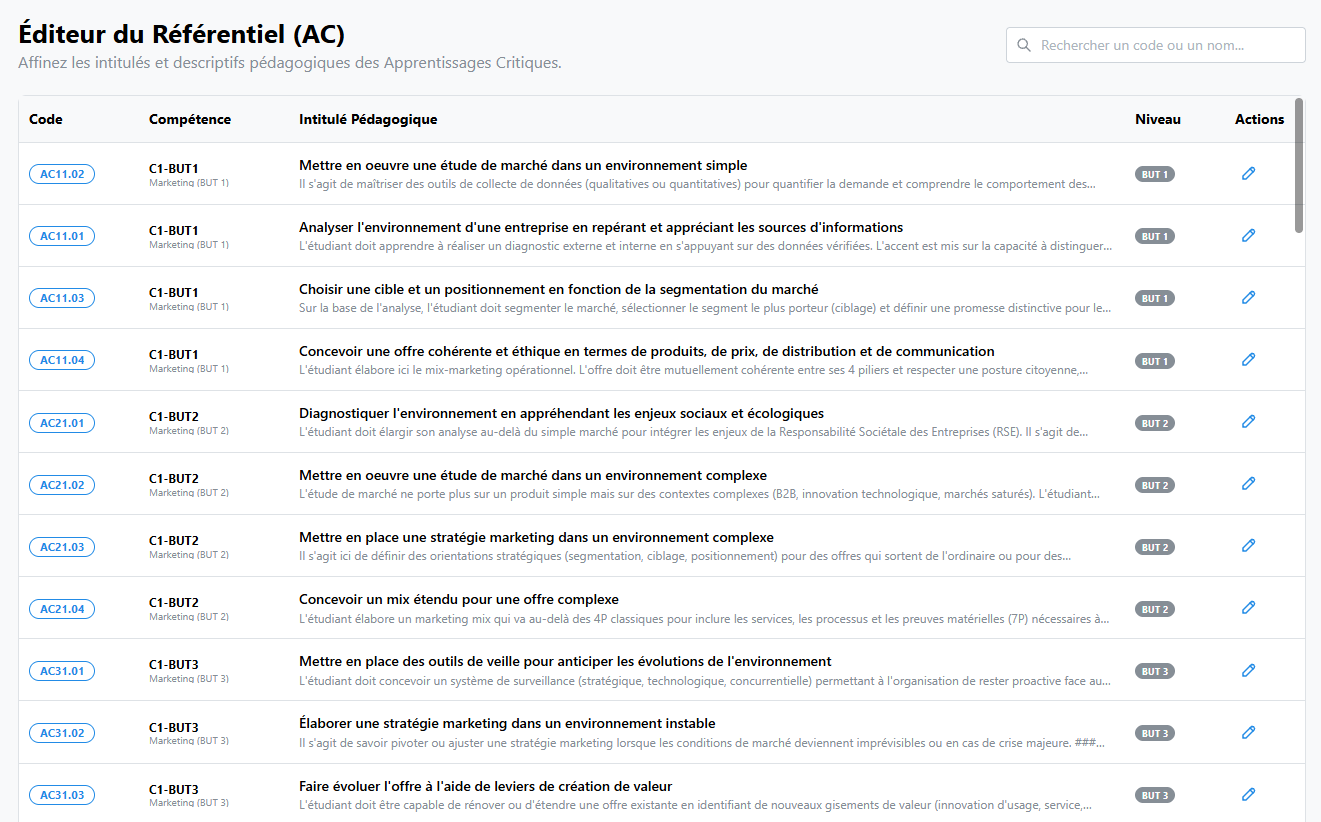
\includegraphics[width=0.85\textwidth]{5}}
    \caption{Éditeur des Apprentissages Critiques}
\end{figure}

\subsection{Découverte \& Fiches PDF}
Pour l'analyse et l'archivage :
\begin{itemize}
    \item \textbf{Découverte :} Visualisez les liens logiques entre les cours et les compétences.
    \item \textbf{Fiches PDF :} Générez en un clic les syllabus officiels pour l'administration ou les étudiants.
\end{itemize}

\begin{figure}[H]
    \centering
    \fbox{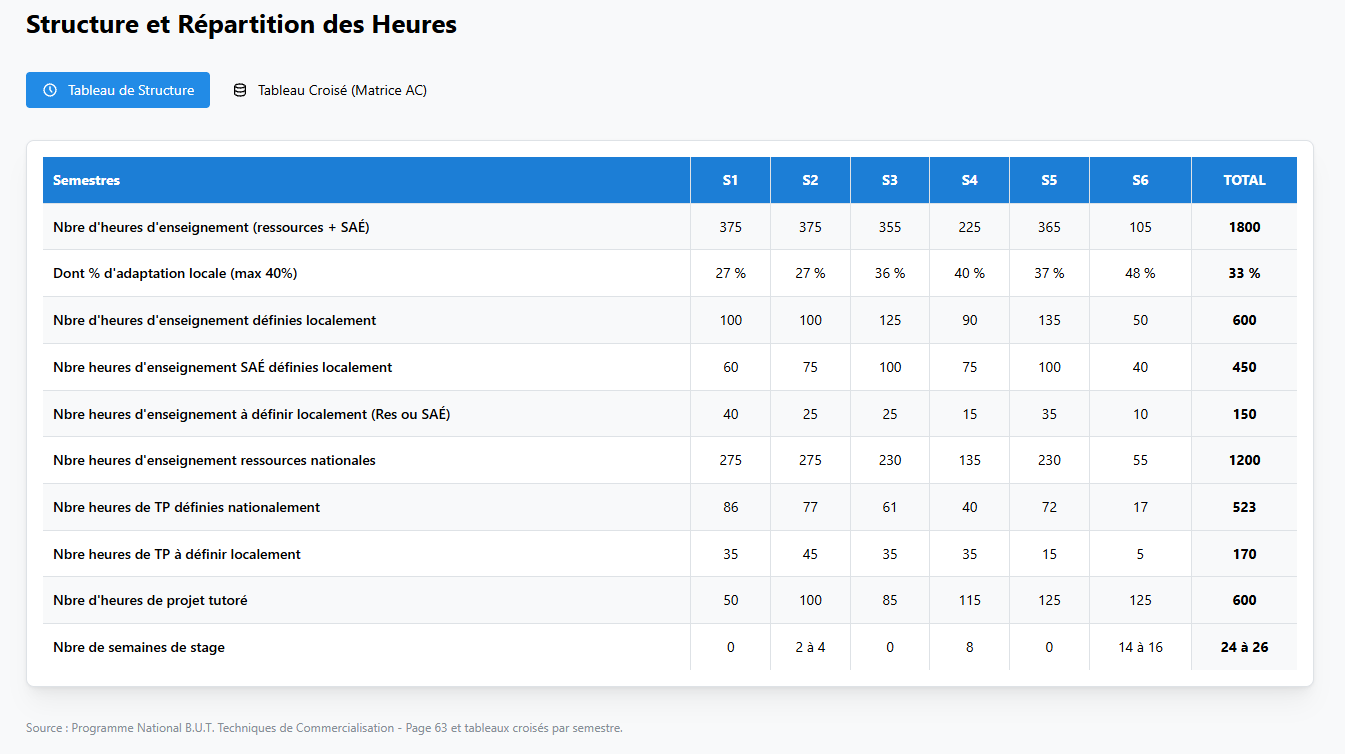
\includegraphics[width=0.45\textwidth]{6}} \hfill
    \fbox{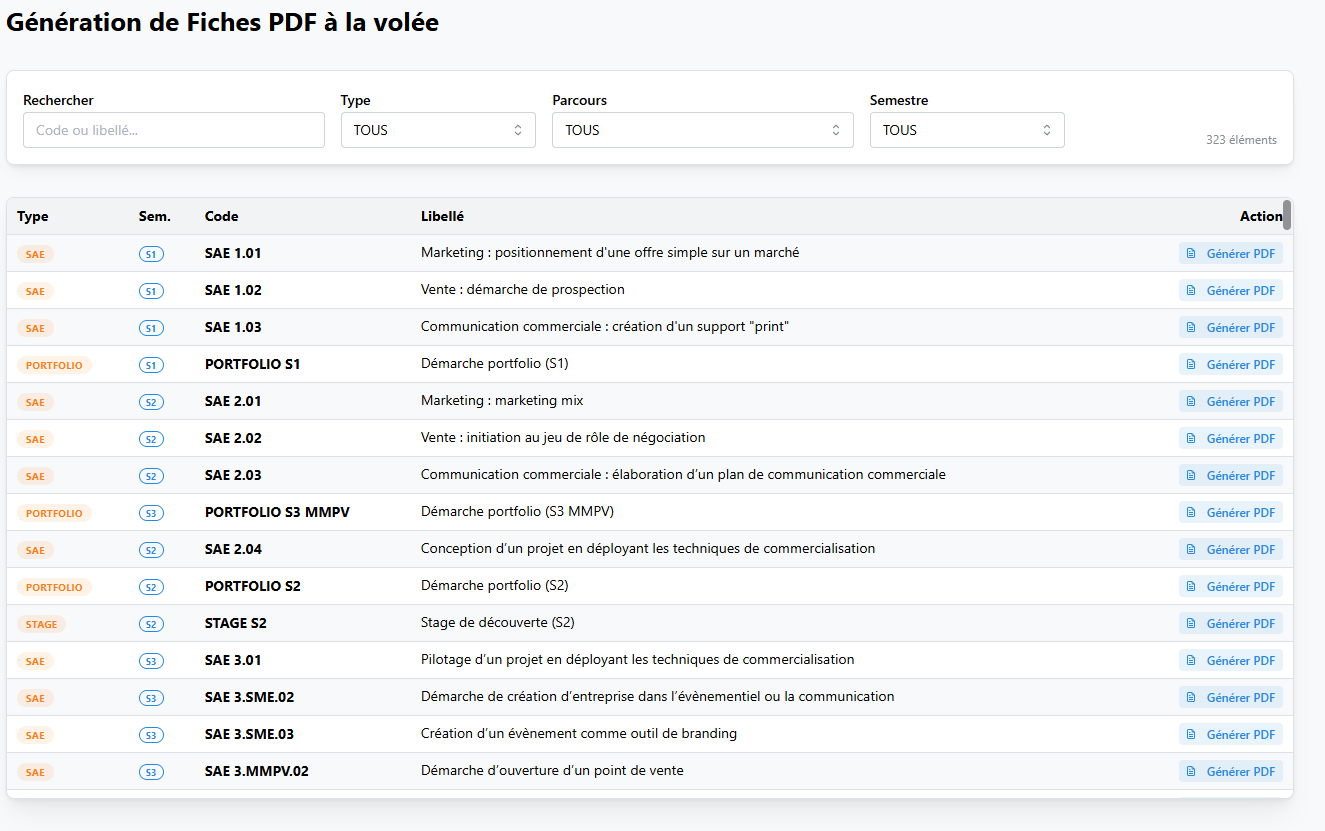
\includegraphics[width=0.45\textwidth]{7}}
    \caption{Outils de visualisation et d'export}
\end{figure}

\newpage
\section{Le Bloc Outils Enseignant}
C'est ici que se fait le travail de suivi quotidien des étudiants.

\subsection{Suivi des Stages \& Workflow}
Le module \textbf{Tutorat} automatise le cycle de vie du stage. Plus qu'un simple annuaire, c'est un outil de dialogue entre l'étudiant, le tuteur académique et le tuteur pro.

\begin{figure}[H]
    \centering
    \fbox{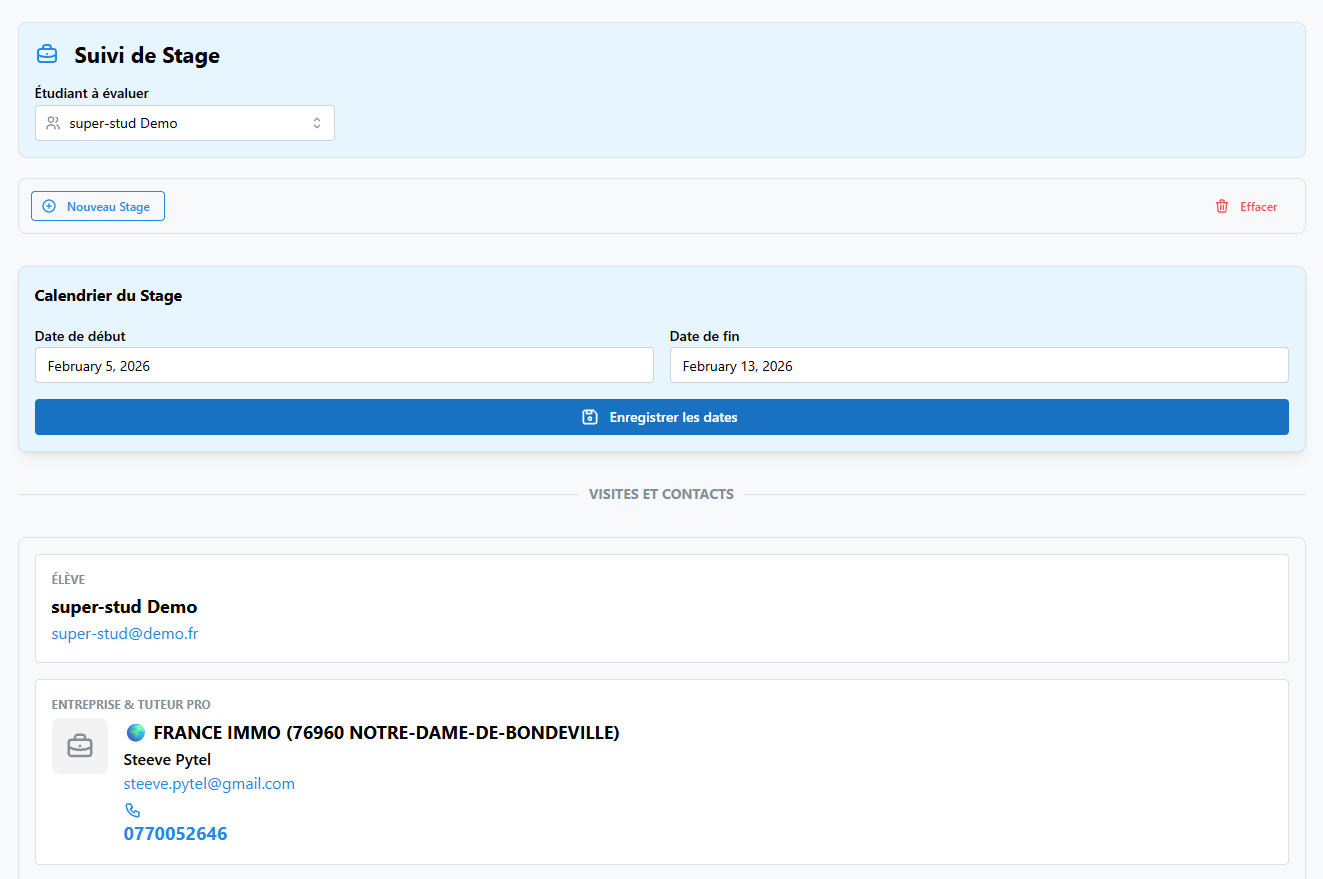
\includegraphics[width=0.85\textwidth]{8}}
    \caption{Interface de pilotage des stages}
\end{figure}

\textbf{Le cycle de validation en 5 étapes :}
\begin{enumerate}
    \item \textbf{Déclaration :} L'étudiant saisit ses missions et coordonnées entreprise.
    \item \textbf{Suivi (Visite) :} Le tuteur enseignant consigne son compte-rendu de visite directement dans l'app.
    \item \textbf{Auto-Évaluation :} L'étudiant dépose son rapport et ses "preuves" de réussite dans la médiathèque.
    \item \textbf{Évaluation Pro :} Le tuteur entreprise reçoit un \textbf{lien unique par email}. En un clic, il remplit une grille de savoir-être (soft-skills).
    \item \textbf{Jury :} L'enseignant fait la synthèse et valide les AC correspondants.
\end{enumerate}

\begin{tcolorbox}[colback=blue!5,colframe=primaryBlue,title=Innovation : Le Magic Link]
Le tuteur en entreprise n'a aucun compte à créer. Le lien envoyé par le système lui donne un accès direct et sécurisé à la grille d'évaluation de son stagiaire uniquement.
\end{tcolorbox}

\subsection{Médiathèque des Preuves \& Portfolio}
\textbf{Le cœur du dispositif d'évaluation.} Pour valider un Apprentissage Critique (AC), l'étudiant doit apporter une preuve concrète (livrable, vidéo, témoignage).

\textbf{Intégration Nextcloud / OnlyOffice :}
Skill Hub est couplé à un serveur de fichiers sécurisé. En tant qu'enseignant, vous pouvez :
\begin{itemize}
    \item Parcourir les dossiers de chaque étudiant.
    \item \textbf{Consulter les fichiers en ligne} sans les télécharger (PDF, Word, Excel).
    \item Annoter ou valider directement la preuve.
\end{itemize}

\begin{figure}[H]
    \centering
    \fbox{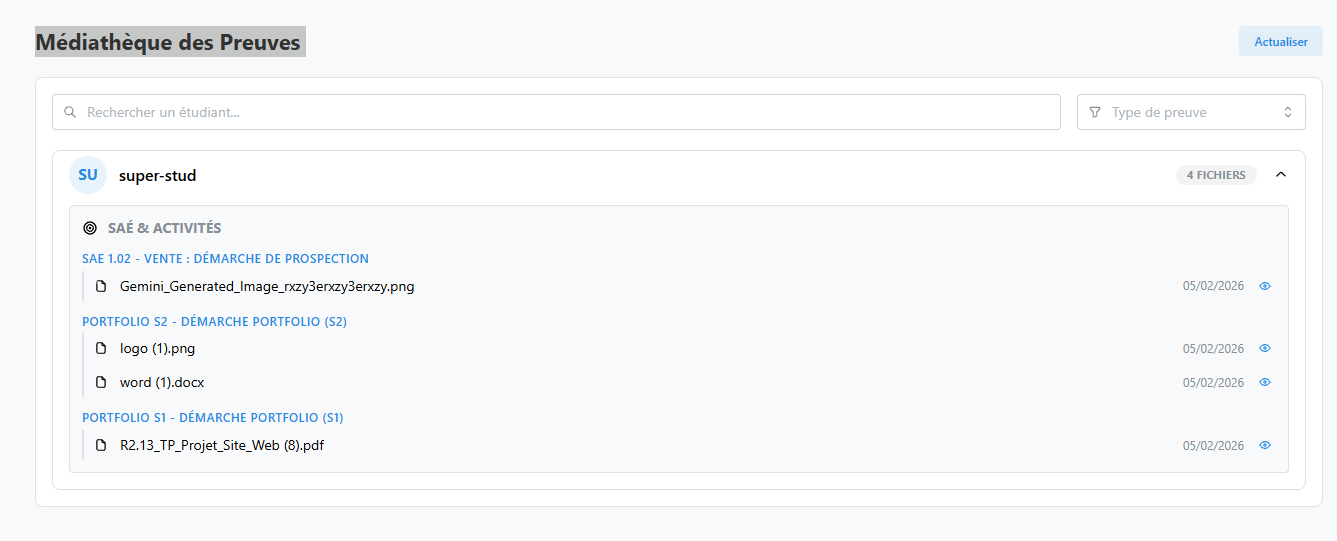
\includegraphics[width=0.85\textwidth]{c}}
    \caption{Consultation fluide des livrables étudiants}
\end{figure}

\begin{infoBox}{L'avis du Tuteur}
La médiathèque permet une traçabilité totale : vous avez sous les yeux les mêmes documents que l'étudiant utilisera lors de sa soutenance de portfolio.
\end{infoBox}

\section{Partenaires et Technologies Internes}
Skill Hub est propulsé par un écosystème de technologies leaders, hébergées souverainement pour garantir la confidentialité des données pédagogiques.

\begin{figure}[H]
    \centering
    \begin{minipage}{0.3\textwidth}
        \centering
        
\includegraphics[height=1.2cm]{logo_nextcloud}
        \caption*{\small Stockage \& Édition}
    \end{minipage}
    \hfill
    \begin{minipage}{0.3\textwidth}
        \centering
        
\includegraphics[height=1.2cm]{logo_mattermost}
        \caption*{\small Collaboration}
    \end{minipage}
    \hfill
    \begin{minipage}{0.3\textwidth}
        \centering
        
\includegraphics[height=1.2cm]{logo_mistral}
        \caption*{\small Intelligence Artificielle}
    \end{minipage}
\end{figure}

\newpage
\section{Assistance \& Support}

\subsection{Assistant IA}
Une question sur le programme ? Besoin de retrouver un code module ?
L'\textbf{Assistant IA}, basé sur la technologie \textbf{Mistral AI}, est disponible 24/7 pour répondre à vos questions sur le contexte pédagogique du département.

\begin{figure}[H]
    \centering
    \fbox{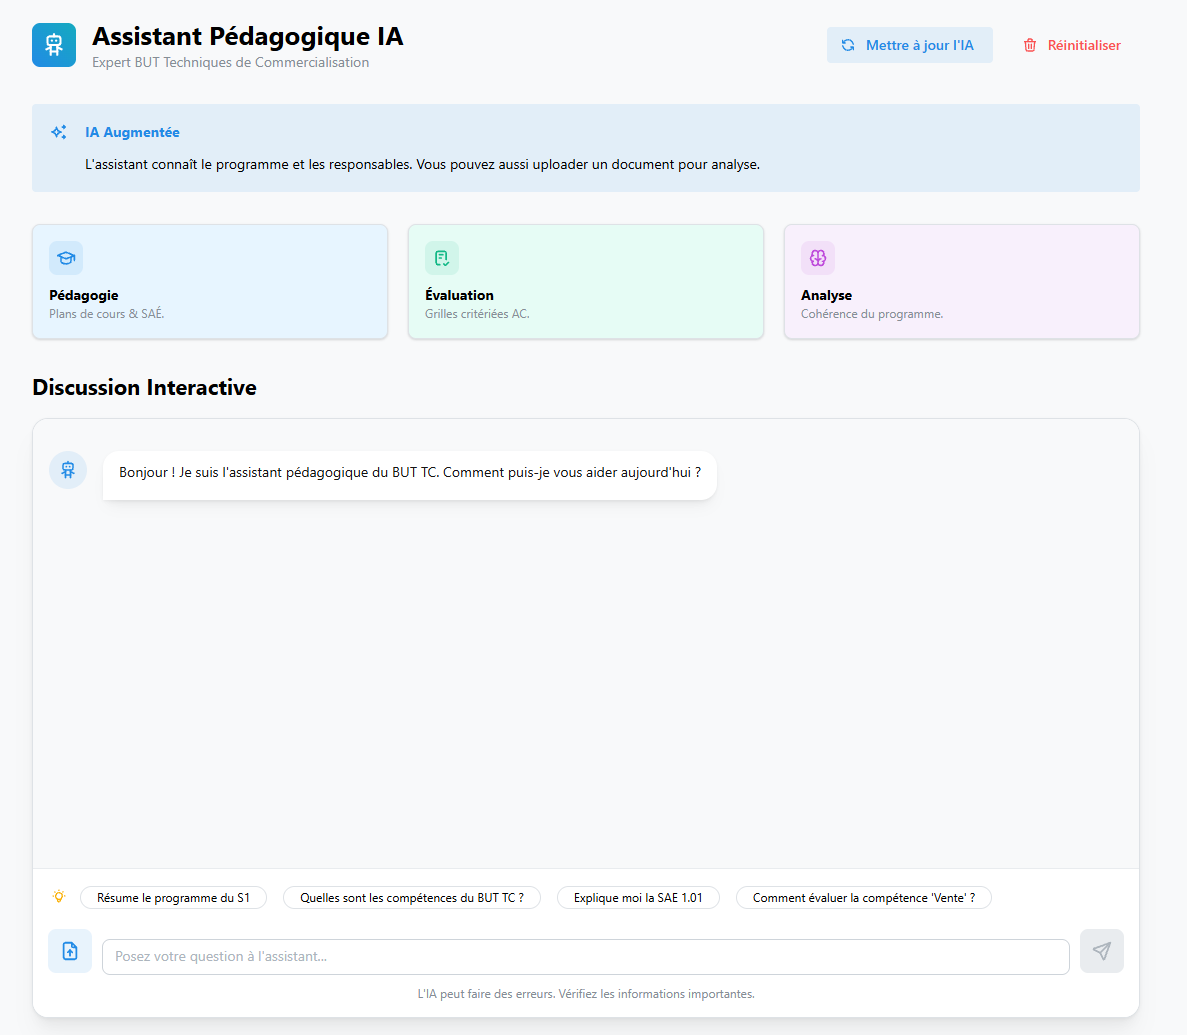
\includegraphics[width=0.85\textwidth]{b}}
    \caption{Chat avec l'Assistant Pédagogique}
\end{figure}

\newpage
\section{Le Bloc Idées \& Outils}
Ce dernier bloc regroupe des utilitaires de communication et de collaboration pour l'équipe pédagogique.

\subsection{Boîte à Idées}
Votre avis compte. Utilisez la \textbf{Boîte à Idées} pour :
\begin{itemize}
    \item Signaler un bug.
    \item Suggérer une amélioration.
    \item Demander une nouvelle fonctionnalité.
\end{itemize}

\begin{figure}[H]
    \centering
    \fbox{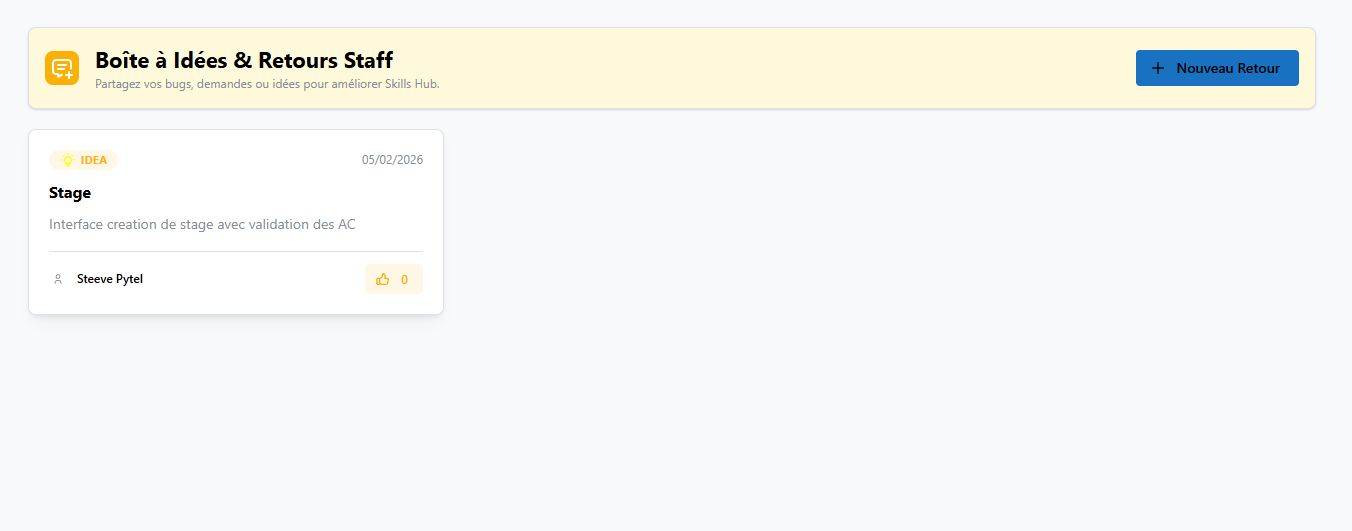
\includegraphics[width=0.85\textwidth]{d}}
    \caption{Nous contacter via la Boîte à Idées}
\end{figure}

\begin{infoBox}{Contact direct}
Pour toute question spécifique ou demande d'accompagnement, vous pouvez contacter : \\
\centerline{\textbf{Steeve Pytel} : \href{mailto:steeve.pytel@univ-lehavre.fr}{steeve.pytel@univ-lehavre.fr}}
\end{infoBox}

\end{document}